\chapter{Violazioni del Modello Lineare Classico}

\subsection{Eteroschedasticità}
L'ipotesi di omoschedasticità suppone che il termine di errore sia uguale per tutte le variabili indipendenti, quindi dato un certo valore di X lo spread nella distribuzione delle Y è sempre lo stesso, come si può vedere dalla figura \ref{fig:regressione-omoschedastica}.
\begin{figure}[H]
	\centering
	\makebox[\textwidth]{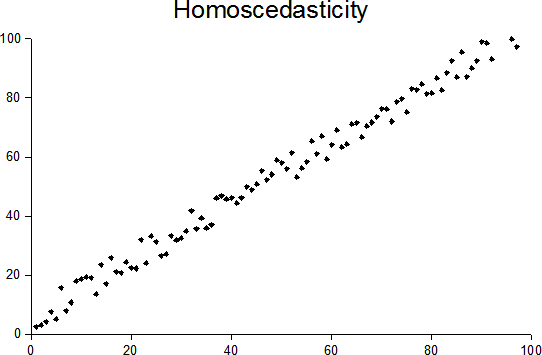
\includegraphics[width=0.8\textwidth]{Immagini/Homoscedasticity.png}}
	\caption{Regressione lineare con distribuzione omoschedastica degli errori.}
	\label{fig:regressione-omoschedastica}
\end{figure} 
ovvero $Var(\varepsilon \vert x_i) = \sigma^2$ e $E(y \vert x) = 0$.

Al contrario ci possono essere situazioni in cui il termine di errore varia tra le diverse variabili indipendenti, ottenendo così la situazione mostrata in figura \ref{fig:regressione-eteroschedastica}
\begin{figure}[H]
	\centering
	\makebox[\textwidth]{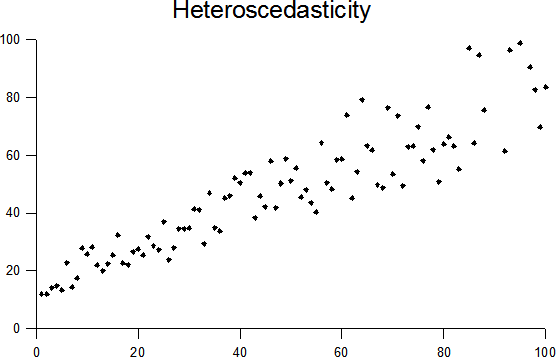
\includegraphics[width=\textwidth]{Immagini/Heteroscedasticity.png}}
	\caption{Regressione lineare con distribuzione eteroschedastica degli errori.}
	\label{fig: regressione-eteroschedastica}
\end{figure} 
Questo andamento è conseguenza del fatto che la varianza del termine di errore, stimato dai residui del modello, dato un certo valore di X non è più costante e in particolare ora dipende da X.

Un altro andamento anomalo del tipo in figura \ref{fig: residui-eteroschedastici} lo si può osservare in un semplice grafico scatter plot della variabile dipendente in funzione della variabile indipendente: nel caso di errori omoschedastici i punti sono collocati in modo equidistante dalla retta interpolante, mentre nel caso di errori eteroschedastici i punti sono distanziati in maniera diversa da questa. Il problema nel caso eteroschedastico si pone in quanto il metodo OLS dei minimi quadrati ordinari mira a minimizzare i residui ottenendo lo standard error minimo. Il metodo OLS pesa però tutte le osservazioni allo stesso modo, mentre quando si trattano errori eteroschedastici è necessario pesare meno i valori con più errore e pesare di più quelli che invece sono più rilevanti.\\
Se utilizziamo ancora stimatori OLS cosa succede?\\
$\rightarrow$ Gli stimatori OLS dei parametri sono ancora unbiased, consistenti e distribuiti in modo asintoticamente normale. \textit{Non} sono più stimatori \textit{efficienti} tra tutti gli stimatori possibili dei parametri che sono lineari e unbiased in $Y$, dato un certo valore di $X$. In generale quindi possiamo dire che non sono più BLUE (Best Linear Unbiased Estimator).
La statistica t di Student calcolata in base al valore della deviazione standard utilizzato nel metodo OLS, non risulta più distribuita in modo normale nemmeno per grandi campioni se l'errore è eteroschedastico. Questo avviene principalmente per due ragioni:
\begin{enumerate}
	\item Le stime campionare tendono a sottostimare il valore della varianza.
	\item Non c'è più da calcolare una sola varianza ma diverse varianze.
\end{enumerate}
Come conseguenza della sottostima della varianza si ha che la statistica t di Student ha valori erroneamente elevati, si possono considerare come significativi paramentri che in realtà non lo sono. Per lo stesso motivo la regione di accettazione diventa molto più piccola di quanto non lo sia in realtà e di conseguenza la regione di rifiuto molto grande.
L'ipotesi di omoschedasticità (uguali varianze) è  infatti alla base di test come l'analisi della varianza ANOVA (Analysis Of Variance) e il t-test di Student.
\begin{tcolorbox}[colback=cyan!5!white, colframe=cyan!75!black, title = ANOVA]
	L'analisi della varianza ANOVA è utilizzata per testare differenze tra medie, utilizzando appunto le varianze. Quando le medie sono solamente due è indifferente utilizzare questo test oppure il t-test, mentre si deve usare necessariamente il test ANOVA quado le medie da testare sono più di due.\\
	Dati quindi un insieme di campioni di cui sono stati calcolati media e varianza per ciascuno si può procedere a costruire il test ANOVA, come segue:
	\begin{equation}
	F = \frac{\sigma^2_{between}}{\sigma^2_{within}}
	\label{eq: test ANOVA}
	\end{equation}
	dove $\sigma^2_{between}$ rappresenta la varianza tra gruppi, mentre $\sigma^2_{within}$ quella in gruppi.\\
	La varianza $within$ in gruppi è la media delle varianze di ciascun campione pesata sul numero di gradi di libertà del campione, overo:
	\begin{equation}
	\sigma^2_{within} = \frac{1}{a(n-1)}\sum_{i=1}^{a}\sum_{j=1}^{n}(y_{ij} - \bar{y_i})^2
	\end{equation}
	in cui appunto la $i = 1 \cdots a$ identifica il campione e $j = 1 \cdots n$ identifica invece il numero di osservazione che si sta prendendo in considerazione. Quindi si somma prima su $j$ per calcolare le varianze del campione che si sta considerando, e poi si somma su $j$ per fare la media delle varianze dei campioni, dividendo poi per il peso del campione pari a $n-1$, dove $n$ è il numero delle osservazioni fatte per campione. \\
	La varianza $between$ tra gruppi invece è calcolata a partire dalla devianza totale che è la varianza stimata con tutte le osservazioni di tutti i campioni ovvero come se le varie osservazioni dei vari campioni appartenessero tutte ad un unico campione. A questo punto la varianza tra gruppi si ottiene moltiplicando questa per $n$, ovvero:
	\begin{equation}
	\sigma^2_{between} = \frac{n}{a-1}\sum_{i=1}^{a} (\bar{y_i} - \bar{\bar{y}})
	\end{equation}
	dove $\bar{\bar{y}}$ rappresenta appunto la media ottenuta considerando le osservazioni di tutti i campioni, mentre le $\bar{y}_i$ sono le medie dei singoli campioni.	
	Si può quindi a questo punto effettuare il test in \eqref{eq: test ANOVA}. Poichè le due varianze rapportate sono stime di una stessa varianza parametrica (quella della distribuzione vera se si conoscesse tutta la popolazione), allora questo rapporto deve essere uguale a 1 in teoria. Se però i campioni provengono da popolazioni diverse si ottiene un valore al numeratore più grande rispetto al denominatore, risultando così in un numero maggiore di 1.\\
	Per ogni combinazione di gradi di libertà di numeratore e denominatore, si confronta il valore ottenuto con la distribuzione di una variabile casuale distribuita come una F di Sendecor con pari gradi di libertà. Stabilendo il livello di confidenza, si confronta con il valore tabulato della $F$ e si decide se confermare l'ipotesi nulla, cioè che le medie provengono tutte da una stessa distribuzione, oppure se rigettarla, affermando quindi che almeno una non appartiene alla distribuzione delle altre.	
	[ref:http://docenti.unimc.it/monica.raiteri/teaching/2013/12316/files/slides-i-parte-per-studenti-frequentanti/interpretazione-del-test-f-distribuzione-f-di]
\end{tcolorbox}
Oltre alla visualizzazione grafiche, l'eteroschedasticità si può individuare anche tramite metodi analitici, ovvero eseguendo dei test come il \textit{test di White} o il \textit{test di Breuch-Pagan}.
\subsubsection{Test di White}
Il test di White testa l'ipotesi nulla di omoschedasticità degli errori:
\begin{equation}
H_0 = Var(\epsilon \vert X) = \sigma^2 \cdot I_n
\end{equation}
e ovviamente ha come ipotesi alternativa la stessa espressione sopra in cui vale però una disuguaglianza.
Il test di White si basa su na regressione OLS dei residui, ovvero:
\begin{enumerate}
	\item si stima il modello lineare con il metodo OLS ottenendo:
	\begin{equation}
	\hat{Y_i} = \hat{\beta_0} + \hat{\beta_1} \cdot X_{i1} + \cdots + \beta_n \cdot X_{in} + \hat{\epsilon_i}
	\end{equation}
	\item si fa una regressione OLS  sugli errori assumendo che l'eteroschedasticità possa essere una funzione lineare dei regressori, del loro quadrato o della loro interazione $x_{ij}\cdot x_{ij}$. Quindi si ottiene:
	\begin{equation}
	\hat{\epsilon}_i^2 = \delta_0 + \delta_1 \hat{Y}_i + \delta_2 \hat{Y}_i^2
	\end{equation}
	dove appunto si utilizza il risultato della regressione del modello lineare effettuato all'inizio. Considerando i quadrati si considerano tramite i doppi prodotti anche i termini di interazione.
	\item si calcola $R^2_{\hat{\epsilon}_i^2}$
	\item si effettua il test LM, definito come segue:
	\begin{equation}
	LM = nR^2_{\hat{\epsilon}_i^2}
	\end{equation}
	che si distribuisce come un $\chi^2$ con un numero di gradi di libertà pari al numero di regressori inseriti nel modello.
	\item scelto un livello di significatività $\alpha$ l'ipotesi nulla sarà rigettata se il test $LM$ risulta superiore al valore soglia di $\chi^2$ (tabulato), che è associato al livello di significatività scelto.
\end{enumerate}
\subsubsection{Test di Breusch-Pagan}
Il test di Breuch Pagan a differenza del test di White ipotizza che l'eteroschedasticità sia solamente una funzione lineare delle variabili indipendenti, trascurando quindi i termini quadratici e di interazione. Si procede quindi nello stesso modo definito precedentemente in cui però si assume che la forma funzionale per $\epsilon$ sia:
\begin{equation}
\hat{\epsilon}_i^2 = \delta_0 + \delta_1\hat{Y}_i
\end{equation}
CHIEDERE..
\subsection{Autocorrelazione}
A volte è possibile che gli errori (e quindi i residui) siano correlati tra loro, soprattutto in serie storiche o territoriali è ragionevole ipotizzare che ci sia correlazione tra gli errori che vengono stimati in momenti successivi o territori vicini.\\
Nel modello lineare classico si suppone che:
\begin{equation}
Cov(\varepsilon_i, \varepsilon_j) = 0 \quad \forall i \neq j
\end{equation}
Quando ciò non si verifica si dice che gli erroi sono correlati o che si è in presenza di una correlazione seriale. Se c'è omoschedasticità ma c'è correlazione, la matrice degli errori è:
\begin{equation}
\Sigma = \begin{pmatrix}
\sigma^2 & \rho_{1,2} & \cdots & \rho_{1,n} \\ 
\rho_{1,2} & \sigma^2 & \cdots & \vdots \\ 
\vdots &  & \ddots & \vdots \\ 
\rho_{1,n} & \cdots & \cdots & \sigma^2
\end{pmatrix} 
\end{equation}
dove i vari $\rho$ rappresentano i termini di correlazione dei vari termini di errore tra loro. La matrice ovviamente risulta simmetrica.
L'errore può essere correlato con quello dell'osservazione immediatamente precedente e quindi avere una correlazione di primo livello, oppure ci può essere una correlazione di secondo livello o livello maggiore se gli errori correlati sono distanti due o più osservazioni. Ciò è espresso con la seguente formula:
\begin{equation}
\varepsilon'_i = \varepsilon'_{i-1} + \eta_j
\end{equation}
dove si è utilizzata la notazione primata per identificare il fatto che gli errori sono correlati tra loro e non sono più sferici. Gli $\eta_j$ sono invece identicamente e indipendentemente distribuiti in modo normale con $N(0,\sigma_i)$ per rappresentare quindi la parte di correlazione dell'errore con sè stesso (la diagonale della matrice).\\
Si ha autocorrelazione \textit{positiva} quando residui consecutivi tendono ad essere dello stesso segno e simili in valore, \textit{negativa} quando invece residui consecutivi sono di segno differente.
IMMAGINI AUTOCORRELAIZONE POSITIVA E NEGATIVA
In caso di autocorrelazione gli stimatori OLS  dei parametri per la regressione lineare sono ancora lineari e corretti (unbiased) ma non sono più i migliori stimatori possibili, quindi non sono più BLUE, ovvero esistono altri stimatori che risultano più efficienti. come conseguenza di ciò non si potrà più usare la varianza campionaria nella statistica $t$ perchè non potrà più approssimare la varianza vera in quanto la $t$ è costruita supponendo l'incorrelazione degli errori nella popolazione e il valore atteso della varianza campionaria non stima correttamente la varianza vera. Di conseguenza la statistica $t$ assume valori erroneamente elevati, considerando significativi parametri quando in realtà non lo sono, ovvero si amplia la regione di rifiuto per l'ipotesi nulla con il conseguente restringimento della regione di accettazione. \\
Ragionamenti analoghi si possono fare per il test F, che corrisponde semplicemente al quadrato del t test.
\subsubsection{Individuazione grafica}
Si può notare un autocorrelazione nei reisui osservando:
\begin{enumerate}
	\item scatter plot della vraibile dipendente in funzione in funzione del regressore $x$. Nel caso in cui ci fossero più regressori bisogna fare uno scatter plot in funzione di goni regressore. Se si nota una certa regolarità nell'andamento allora si è in presenza di correlazione.
	\item scatter plot dei residui in funzione del regressore: anche qui valgono le stesse considerazioni fatte sopra. Se i residui oscillano intorno allo zero non c'è correlazione.
	\item Residui in funzione dei residui ritardati
	\item Correlogramma, permette di identificare chiaramente quali sono i gradi di correlazione che influiscono di più. Solitamente nei correlogramma è mostrata anche una banda di confidenza che indica il limite entro il quale non si ritiene che vi sia autocorrelazione. Se il coefficiente di autocorrelazione che si sta valutando esce da questa banda allora si è in presenza di autocorrelazione.
\end{enumerate}
\subsubsection{Test di Durbin-Watson}
Il test di Durbin-Watson verifica l'ipotesi nulla:
\begin{equation}
H_0:\; \rho = Corr(\varepsilon'_i, \varepsilon'_{i-1}) = 0
\end{equation}
dove $\varepsilon'_i$ e $\varepsilon'_{i-1}$ sono i residui relativi all'osservazione i-esima e i-1-esima.\\
La statistica di DW con cui si effettua il test è la seguente:
\begin{equation}
DW = \frac{\sum_{i}(\varepsilon'_i - \varepsilon'_{i-1})^2}{\sum_{i} \varepsilon'^2_{i}} \quad \text{per}\; i = 1 \dots n
\label{eq: DW test}
\end{equation}
La statistica di DW è centrata su 2 ed è sempre compresa tra 0 e 4. Nel caso in cui i residui siano correlati positivamente tende a 0, mentre nel caso in cui siano correlati negativamente tende a 4.\\
Non si conosce la distribuzione teorica di questa statistica, comunque esistono dei valori tabulati in base al numero di regressori, il numero di osservazioni e livello di significatività con cui si vuole valutare l'ipotesi nulla, con in quali è possibile individuare dei valori critici $d_l$ e $d_u$ che delimitino le regioni di rifiuto e di accettazione. Se il valore che si trova dalla statistica in \eqref{eq: DW test} è $d < d_l$ allora si può concludere che c'è autocorrelazione positiva, se $d > d_u$ allora si può concludere che c'è autocorrelazione negativa, mentre se $d$ è compreso tra questi due valori allora non c'è sufficiente evidenza per concludere che ci sia autocorrelazione tra i residui. Convenzionalmente, nel caso in cui i valori di $d_l$ e $d_u$ non vengano specificati si fissa $d_l = 1$ e $d_u = 3$.
\section{WLS e GLS}
Per tenere conto di eteroschedasticità e correlazione nei residui si possono applicare due metodi: il metodo dei minimi quadrati pesati WLS e il metodo dei minimi quadrati generalizzati GLS.
\subsection{Il metodo WLS}
Per tenere conto dell'eteroschedasticità, e fare in modo che i valori stimati dei parametri $\hat{\beta}$ siano ancora gli stimatori migliori, è stato dimostrato che tali stimatori risultano ancora i migliori se si minimizza una somma pesata dei residui dove i pesi sono il reciproco dello scarto quadratico medio per i valori previsti, ovvero:
\begin{equation}
S = \sum_{i=1}^{n} \sqrt{W_{ii}} r_i^2 \quad \text{dove}\quad W_{ii} = \frac{1}{\sigma_i^2} 
\label{eq: somma-gls}
\end{equation}
per poi procedere con la minimizzazione come nel caso OLS. \\
Alternativamente al posto di definire la \eqref{eq: somma-gls} si può effettuare un cambiamento di variabili per il modello lineare classico, ovvero passare da:
\begin{equation}
Y = X\beta + \varepsilon^\star
\label{eq: regressione-lineare-eterosched}
\end{equation} 
dove $\varepsilon^\star$ indica l'errore eteroschedastico, a:
\begin{equation}
Y^\star = X^\star\beta + \varepsilon
\end{equation}
dove:
\begin{equation}
\begin{split}
Y^\star &= \frac{Y}{\sqrt{W_{ii}}} \\
X^\star &= \frac{X}{\sqrt{W_{ii}}} \\
\end{split}
\end{equation}
ovvero si dividono entrambi i membri dell'equazione OLS per $W_{ii}$ e poi si procede con il metodo dei minimi quadrati ordinari. Questa volta l'errore risulta omoschedastico, in quanto abbiamo diviso per la devianza standard della media anche la parte di errore, quindi la diagonale della matrice di correlazione REFF A UNA MATRICE PRECEDENTE DI CORRELAZIONE DEI RESIDUI NEL CASO DI ERRORI ETEROSCHED (FARLA NEL CASO MANCHI) dei residui non è più composta da termini tutti diversi tra loro ma saranno tutti uguali e costanti.
\subsection{Il metodo GLS}
Anche il metodo GLS, di cui il metodo WLS è un caso particolare, si basa su una trasformazione di variabili.
Data la matrice di varianza e covarianza per gli errori del modello lineare classico, caratterizzata, nel caso di errori omoschedastici ma correlati, da una diagonale tutta uguale e con termini diversi da zero fuori dalla diagonale, si supponga che esista una matrice $V$ tale che:
\begin{equation}
\Sigma_{\varepsilon^\circ} = V \sigma^2 V^t
\label{eq: matrice-GLS}
\end{equation}
o analogamente:
\begin{equation}
\Sigma_{\varepsilon^\circ}^{-1} = (V)^{-1} \frac{1}{\sigma^2} (V^t)^{-1}
\end{equation}
dove si è usata la notazione $\varepsilon^\circ$ per indicare che gli errori sono correlati.\\
Si possono definire gli errori trasformati, fatti nel seguente modo:
\begin{equation}
\varepsilon = V^{-1} \varepsilon^\circ
\end{equation}
poichè vale la \eqref{eq: matrice-GLS}, allora si ottiene:
\begin{equation}
\Sigma_\varepsilon = VV^{-1} \sigma^2 (V^t)^{-1}V^t = \sigma^2 \cdot I_n
\end{equation}
A questo punto se passiamo sin da subito a delle variabili trasformate nel modello, moltiplicando a entrambi i membri l'equazione del modello lineare classico in \eqref{eq: regressione-lineare-eterosched}, considerando di avere questa volta errori autocorrelati omoschedastici, per $V^{-1}$, si può applicare il metodo OLS classico per ottenere i parametri.
La matrice $V$ si può ottenere tramite decomposizione spettrale della matrice $\Sigma_\varepsilon$ di correlazione degli errori.
Lo stimatore GLS che si calcola in questo modo assegna un peso maggiore alle variabili caratterizzate da una minore varianza e quindi da considerarsi più attendibili. Inoltre lo stimatore è consistente, corretto (unbiased) e per il terorema di Aitken (analogo al Gauss-Markov per gli OLS) si dimostra che è anche efficiente.
\subsubsection{Procedimento}
Prima di procedere alla costruzione delle stime GLS,  si deve stimare il l'errore autocorrelato e i vari livelli di autocorrelazione. A questo scopo si costruisce un modello di regressione che spiega l'errore $\varepsilon_i$ per l'osservazione i-esima in termini delle variabili esplicative e del residuo ritardato $\varepsilon_{i-1}$, ovvero:
\begin{equation}
\varepsilon^\circ = a_0 + a_1x_1 + \cdots + a_n x_n + a_\varepsilon \varepsilon_{i-1}^\circ
\end{equation}
Il coefficiente di regressione $a_\varepsilon$ che si ottiene rappresenta una stima per il coefficiente $\rho$ di autocorrelazione al primo ordine.
COSA DEL SOTTRARRE (slide 78-79 violazione errori.pptx)
Alternativamente a questo metodo si può utilizzare un metodo autoregressivo che introduce tre le variabili esplicative anche un termine di errore ritardato che tenga conto dell'autocorrelazione al primo ordine. Se ci sono correlazioni anche a ordini successivi si introducono tante variabili esplicative che ne tengano conto in un numero pari agli ordini che si considerano.
\subsection{Il metodo FLGS}
Il problema del metodo GLS è che si basa su una conoscenza perfetta della matrice $\Sigma_\varepsilon$ che però non sempre è nota, per questo si usa il metodo FGLS che si basa sulla matrice di varianza e covarianza campionaria. Gli stimatori che si calcolano con il FGLS sono consistenti nel senso che per $N \rightarrow +\infty \; \Rightarrow \; S_\varepsilon \rightarrow \Sigma_\varepsilon$, dove $S_\varepsilon$ indica la matrice di varianza e covarianza per gli errori campionaria.
\textit{Oss.}\\
Poichè il WLS è un caso particolare del GLS, tutte le procedure che si usano nel GLS si possono adottare anche nel WLS. 
